\subsection{Exp. 3: Paraphrasing Chunks}
\label{subsec:paraphrasing_chunks}

We designed this experiment to evaluate whether chunk-to-chunk paraphrases exhibit better control than text-to-text paraphrases, since chunks contain fewer topic changes than whole texts in theory.
We use five texts from the \dataBlog{}, \dataGutenberg{}, and the \dataStudent{} dataset, respectively.


\begin{figure}[htbp]
  \centering
  \includesvg[width=\linewidth]{images/paraphrasing/experiments/chunks/setup/chunk_api_calls.svg}
  \caption{Breakdown of individual hyperparameters in the paraphrase configuration.
  We use one document per dataset, chunked into one to five sections and paraphrased with all nine paraphrasers in two variance inducing settings (i.e. prompt for one-step, temperature for two-step) versions.
  This amounts to a total of 936 API calls. 
  }
  \label{fig:chunks_api_calls}
\end{figure}


First, texts are chunked preserving sentences.
Chunks are filled with sentences in sentence order that each chunk roughly contains the same number of words.
Second, paraphrase configurations are defined.
Each one-step paraphraser is paired with two prompts, while each two-step paraphraser is paired with two temperatures.
Third, each chunk is paraphrased with all configurations.
These steps account for a minimum of 936 API calls for paraphrasing.
Each component of the configuration is displayed in \autoref{fig:chunks_api_calls}.
Finally, for each paraphrase, we compute BLEU, ROUGE1, ROUGE2, ROUGEL, ROUGELsum, METEOR, BERTScore Precision, BERTScore Recall, BERTScore F1, SBERT \ac{wms}, SBERT cosine similarity.
Scores for chunks of a text are averaged per configuration to obtain the final score for a text configuration pair.
The adequat formula is given in \autoref{eq:avg_chunks} and an example is illustrated in \autoref{fig:mean-bleu}.

\begin{equation}
    score(t) = \frac{1}{\#\text{ chunks}}\sum_{i=1}^{\#\text{ chunks}}score(c_i)\text{, for chunk }c_i \in \text{text }t
\label{eq:avg_chunks}
\end{equation}

\begin{figure}[ht]
  \centering
\resizebox{\textwidth}{!}{%
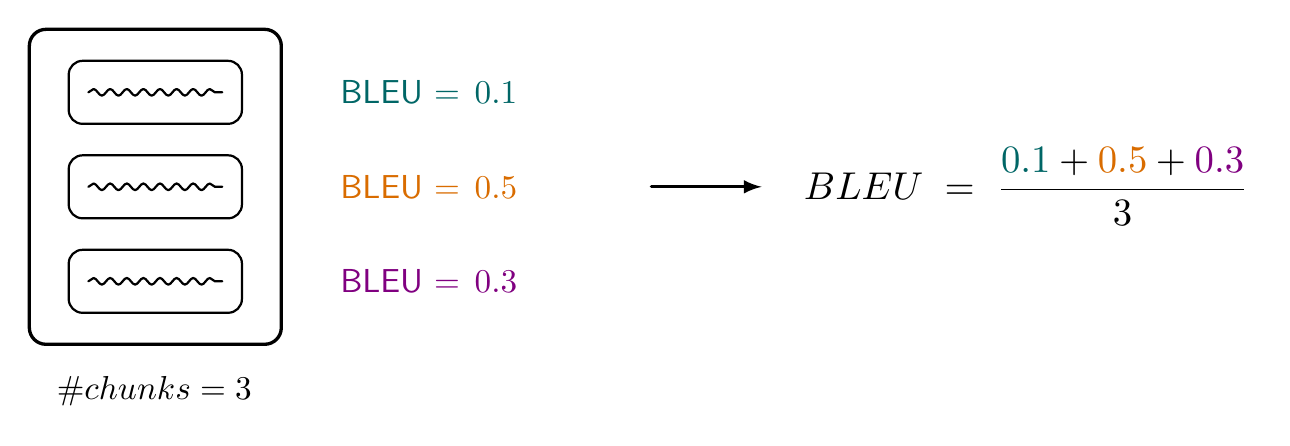
\begin{tikzpicture}[line join=round,line cap=round, >=latex, font=\sffamily]

% --- Left black container with three chunks ---
\draw[black, very thick, rounded corners=6pt]
  (-0.2,3.6) rectangle (3.0,-0.4);

% three inner rounded rectangles
\foreach \y in {2.8,1.6,0.4}{
  \draw[black, thick, rounded corners=5pt] (0.3,\y+0.4) rectangle (2.5,\y-0.4);
  % squiggle inside
  \draw[black, thick, decorate, decoration={snake,amplitude=1.2pt,segment length=6pt}]
    (0.55,\y) -- (2.25,\y);
}

% --- Colored BLEU labels next to each chunk ---
\node[anchor=west, text=teal!80!black, scale=1.2]  at (3.6,2.8) {BLEU $=\,0.1$};
\node[anchor=west, text=orange!85!black, scale=1.2] at (3.6,1.6) {BLEU $=\,0.5$};
\node[anchor=west, text=violet, scale=1.2]         at (3.6,0.4) {BLEU $=\,0.3$};

% --- n_chunks = 3 (black) ---
\node[anchor=west, text=black, scale=1.2] at (0.0,-1.0) {$\#\text{ chunks}=3$};

% --- Arrow to the right and mean BLEU expression ---
\draw[black, very thick, ->, >=latex] (7.7,1.6) -- (9.1,1.6);

\node[anchor=west, text=black, scale=1.4] at (9.3,1.6)
  {$\varnothing\ \text{BLEU} \;=\; \displaystyle
   \frac{\textcolor{teal!80!black}{0.1}+\textcolor{orange!85!black}{0.5}+\textcolor{violet}{0.3}}{3}$};

\end{tikzpicture}
}
  \caption{Computation of the mean \ac{bleu} score over 3 text chunks.}
  \label{fig:mean-bleu}
\end{figure}


\begin{figure}[h!]
    \centering
    \resizebox{\textwidth}{!}{%
        \begin{tikzpicture}[scale=1.2, transform shape, node distance=2cm and 1.5cm]

        % Cylinder (Chunks)
        \begin{scope}[shift={(0,0)}]
          \draw[thick] (0,0) ellipse (0.6 and 0.2); % top ellipse
          \draw[thick] (-0.6,0) -- (-0.6,-1.2);
          \draw[thick] (0.6,0) -- (0.6,-1.2);
          \draw[thick] (0.6,-1.2) arc (0:180:0.6 and 0.2); % bottom ellipse (visible)
          \draw[dashed, thick] (0.6,-1.2) arc (0:-180:0.6 and 0.2); % dashed hidden part
          \node at (0,-1.5) {3x};
        \end{scope}
        \node at (0,0.6) {Chunks};

        % Reference block
        \node[block, right=of {0,-0.6}] (reference) {reference};
        \node[below=0.1cm of reference] {1x};

        % Multiple outputs (Σ=15)
        \node[smallblock, right=0.7cm of reference, yshift=1cm] (b1) {};
        \node[smallblock, below=0.3cm of b1] (b2) {};
        \node[smallblock, below=0.3cm of b2] (b3) {};
        \node[smallblock, below=0.3cm of b3] (b4) {};
        \node[right=0.3cm of b2] (dots) {$\cdots$};
        \node[below=0.1cm of b4] {$\Sigma=15$};

        % Prompt + Temp stacked
        \node[draw, cloud, cloud puffs=10, cloud puff arc=120, minimum width=2.2cm, minimum height=1cm, right=4.5cm of reference] (prompt) {Prompt};
        \node[circle, draw, minimum size=1cm, below=0.8cm of prompt] (temp) {Temp.};
        \node[below=0.1cm of temp] {2x};

        % Paraphrasers
        \node[person, right=3cm of temp, yshift=0.6cm] (p1) {};
        \node[person, right=0.8cm of p1] (p2) {};
        \node[person, right=3cm of temp, yshift=-1.2cm] (p3) {};

        \node[above=0.1cm of p1] {5x2};
        \node[below=0.1cm of p3] {4x1};
        \node[above=0.2cm of p2] {Paraphraser};

        % Paraphrases
        \node[block, right=3cm of p2, minimum height=1cm, minimum width=1.2cm] (paraphrases) {};
        \node[below=0.1cm of paraphrases] {Paraphrases};

        % Arrows
        \draw[arrow] (0.7,-0.6) -- (reference.west);
        \draw[arrow] (reference.east) -- (b1.west);
        \draw[arrow] (reference.east) -- (b2.west);
        \draw[arrow] (reference.east) -- (b3.west);
        \draw[arrow] (reference.east) -- (b4.west);
        \draw[arrow] (b2.east) -- (prompt.west);
        \draw[arrow] (prompt.south) -- (temp.north);
        \draw[arrow] (temp.east) -- (p1.west);
        \draw[arrow] (temp.east) -- (p3.west);
        \draw[arrow] (p2.east) -- (paraphrases.west);

        \end{tikzpicture}%
    }
    \caption{Scaled TikZ diagram}
\end{figure}
